\documentclass[a4paper,12pt]{article}
\usepackage[T1]{fontenc}
\usepackage[utf8]{inputenc}
\usepackage[margin=1in]{geometry}
\usepackage{polski}
\usepackage{amsmath,amssymb,amsthm,mathtools}
\usepackage{enumitem,caption,subcaption,float,tikz}

\DeclareMathOperator\OPT{OPT}
\DeclareMathOperator\vin{in}
\DeclareMathOperator\vout{out}
\DeclareMathOperator\vtail{tail}
\DeclareMathOperator\vhead{head}
\DeclareMathOperator\ov{ov}
\DeclareMathOperator\pref{pref}
\DeclarePairedDelimiter\abs{|}{|}

\theoremstyle{definition}
\newtheorem{definition}{Definicja}
\newtheorem{theorem}{Twierdzenie}
\newtheorem{lemma}{Lemat}

\newcommand{\DrawGadget}{
  \node (outi) at (0,2.5) {$\vout_i$};
  \node (tailij) at (3,3) {$\vtail_{(i,j)}$};
  \node (headij) at (6,3) {$\vhead_{(i,j)}$};
  \node (inj) at (9,2.5) {$\vin_j$};
  \node (ini) at (0,0.5) {$\vin_i$};
  \node (headji) at (3,0) {$\vhead_{(j,i)}$};
  \node (tailji) at (6,0) {$\vtail_{(j,i)}$};
  \node (outj) at (9,0.5) {$\vout_j$};
  \node (iij) at (3,1.5) {$i_{\{i,j\}}$};
  \node (jij) at (6,1.5) {$j_{\{i,j\}}$};
  \draw (tailij) edge (outi) edge (iij) edge (headij);
  \draw (headij) edge (jij) edge (inj);
  \draw (headji) edge (ini) edge (iij) edge (tailji);
  \draw (tailji) edge (jij) edge (outj);
}

\title{Algorytm 2/3-aproksymacyjny dla \textsc{Max-ATSP} i 5/2-aproksymacyjny dla najkrótszego nadsłowa}
\author{Krzysztof Potępa}
\date{Maj 2022}

\begin{document}

\maketitle

\section{Wstęp}

W problemie \textsc{Max-ATSP} (\textsc{Max-ATSP-Path}) mamy dany skierowany graf pełny z nieujemnymi wagami na krawędziach i chcemy znaleźć w nim cykl (ścieżkę) Hamiltona o jak największej sumarycznej wadze. Problem ten jest NP-trudny, ale aproksymowalny z dokładnością do multiplikatywnej stałej. Z punktu widzenia algorytmów tekstowych, problem \textsc{Max-ATSP-Path} znajduje zastosowanie w problemie najkrótszego nadsłowa:
\begin{theorem}[\cite{Breslauer1997,Mucha2007}]
  Mając dany algorytm $\alpha$-aproksymacyjny dla \textsc{Max-ATSP-Path}, możemy uzyskać algorytm $\left(\frac{7}{2}-\frac{3}{2}\alpha\right)$-aproksymacyjny dla najkrótszego nadsłowa.
\end{theorem}
Autorzy pracy \cite{Paluch2012} pokazują prosty algorytm 2/3-aproksymacyjny dla problemu \textsc{Max-ATSP}. Algorytm ten konstruuje ścieżkę o wadze równej co najmniej $2/3$ wagi optymalnego cyklu komiwojażera. W połączeniu z powyższym twierdzeniem, daje to algorytm $5/2$-aproksymacyjny dla problemu najkrótszego nadsłowa.

Niech $G = (V, E)$ będzie skierowanym grafem pełnym, z wagami na krawędziach $w(u, v) \geq 0$, dla każdego $(u, v) \in E$. Przez $\OPT$ oznaczać będziemy wagę optymalnego rozwiązania \textsc{Max-ATSP} w grafie $G$.

Pokrycie cyklowe grafu $G$ to podzbiór krawędzi $C \subseteq E$, taki że każdy wierzchołek ma dokładnie jedną wychodzącą i jedną wchodzącą krawędź. Waga pokrycia cyklowego $w(C)$ to suma wag jego krawędzi. Pokrycie cyklowe o największej wadze można znaleźć w czasie wielomianowym przez redukcję do dwudzielnego skojarzenia o największej wadze.

Łatwo zauważyć, że waga najcięższego pokrycia cyklowego jest nie mniejsza niż $\OPT$, ponieważ cykl Hamiltona to szczególny przypadek pokrycia cyklowego. Rozważmy następujący algorytm aproksymacyjny dla ATSP:
\begin{enumerate}[noitemsep]
  \item Znajdź najcięższe pokrycie cyklowe $C$ grafu $G$.
  \item Usuń z każdego cyklu pokrycia najlżejszą krawędź.
  \item Połącz powstałe ścieżki w cykl/ścieżkę komiwojażera w dowolny sposób.
\end{enumerate}
Jeśli najmniejszy cykl (ze względu na liczbę krawędzi) w pokryciu ma rozmiar $k$, to powyższa procedura daje cykl komiwojażera $C$ o wadze co najmniej $\frac{k-1}{k} \cdot w(C) \geq \frac{k-1}{k} \cdot \OPT$. Dzieje się tak, ponieważ z każdego cyklu usuwamy najlżejszą krawędź, więc może ona stanowić co najwyżej $1/k$ wagi cyklu.

Niestety, w ogólności w pokryciu cyklowym mogą wystąpić cykle rozmiaru $2$, więc powyższy algorytm daje jedynie $1/2$-aproksymację dla \textsc{Max-ATSP}. Co więcej, znalezienie najcięższego pokrycia cyklowego bez 2-cykli jest NP-trudne \cite{Blaser2002}.

Główną ideą algorytmu \cite{Paluch2012} jest obserwacja, że jeśli zabronimy 2-cykli, ale zrelaksujemy nieco wymagania czym jest pokrycie cyklowe, to możemy znaleźć takie "pseudo-pokrycie" w czasie wielomianowym. Później autorzy pokazują, że także da się je przekształcić w ATSP o wadze co najmniej $\frac{2}{3}\OPT$.

\section{2/3-aproksymacja dla \textsc{Max-ATSP}}

Zaczniemy od zdefiniowania wspomnianego wcześniej "pseudo-pokrycia" cyklowego:

\begin{definition}
  Niech $\tilde{G} = (\tilde{V}, \tilde{E})$ będzie grafem otrzymanym z $G$ przez zamianę każdej krawędzi $(i, j) \in E$ przez wierzchołek $v_{(i,j)}$ i dwie krawędzie $(i, v_{(i,j)})$ oraz $(v_{(i,j)}, j)$, obydwie z wagą $\frac{1}{2}w(i,j)$. \emph{Pokrycie cyklowe bez 2-cykli, ale z półkrawędziami}, grafu $G$, to podzbiór krawędzi $\tilde{C} \subseteq \tilde{E}$ taki że:
  \begin{enumerate}[nosep,label=(\alph*)]
    \item każdy wierzchołek w $V$ ma dokładnie jedną wychodzącą i wchodzącą krawędź w $\tilde{C}$;
    \item dla każdej krawędzi $(i, j) \in E$, zbiór $\tilde{C}$ albo nie zawiera żadnej krawędzi ze zbioru $\{(i, v_{(i,j)}), (v_{(i,j)}, j), (j, v_{(j,i)}), (v_{(j,i)}, i)\}$, albo dokładnie jedną incydentną do $i$ i jedną incydentną do $j$.
  \end{enumerate}
\end{definition}

Intuicyjnie, sytuacja że do $\tilde{C}$ należą krawędzie $(i, v_{(i,j)})$ i $(v_{(i,j)}, j)$ odpowiada wybraniu skierowanej krawędzi $(i, j)$, tak jak w zwykłym pokryciu cyklowym. Jeśli natomiast do $\tilde{C}$ należą $(i, v_{(i,j)})$ i $(j, v_{(j,i)})$ to możemy myśleć, że do pokrycia wzięliśmy krawędź, która ma dwa początki, i jej waga to średnia wag $w(i,j)$ i $w(j,i)$. Analogicznie, jeśli do $\tilde{C}$ należą $(v_{(i,j)}, j)$ i $(v_{(j,i)}, i)$ to możemy myśleć o krawędzi, która ma dwa końce. Warunek (a) zapewnia, że w każdym wierzchołku jedna krawędź ma początek i jedna koniec.

Jeśli graf ma co najmniej $3$ wierzchołki, to każdy cykl komiwojażera odpowiada pewnemu pokryciu $\tilde{C}$, więc znów waga najcięższego pokrycia jest nie mniejsza niż $\OPT$. Autorzy pracy pokazują, że najcięższe takie pokrycie można znaleźć w czasie wielomianowym, a następnie wykorzystują je by znaleźć trzy zbiory ścieżek o sumarycznej wadze równej $2w(\tilde{C})$. Aby otrzymać $2/3$-aproksymację dla \textsc{Max-ATSP}, wystarczy wziąć zbiór ścieżek o największej wadze i połączyć jego ścieżki w dowolny sposób.

\begin{lemma}
  Pokrycie cyklowe o największej wadze bez 2-cykli, ale z półkrawędziami, można znaleźć w czasie wielomianowym.
\end{lemma}
\begin{proof}
  Redukujemy problem do problemu najcięższego skojarzenia w grafie $G'$ (niedwudzielnym). Dla każdego wierzchołka $i \in V$, tworzymy w $G'$ wierzchołki $\vin_i$ oraz $\vout_i$. Dla każdej pary krawędzi $(i, j), (j, i) \in E$, tworzymy następujący gadżet:
  \begin{center}
    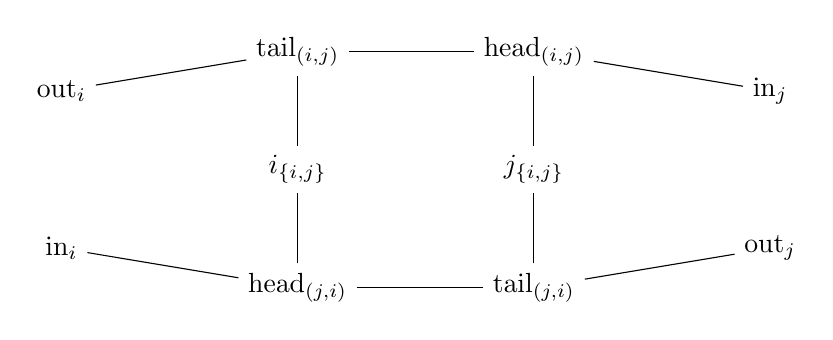
\begin{tikzpicture}
      \DrawGadget
    \end{tikzpicture}
  \end{center}
  W tak skonstruowanym grafie $G'$ szukamy skojarzenia doskonałego $M$ o największej wadze. Mamy następujące możliwości jakie krawędzie zostały skojarzone w pojedynczym gadżecie (z pominięciem symetrycznych przypadków):
  \begin{figure}[H]
    \centering
    \begin{subfigure}[b]{0.48\textwidth}
      \centering
      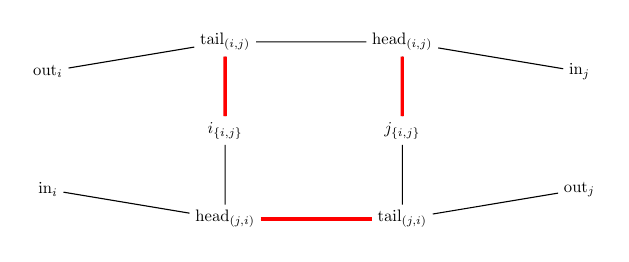
\begin{tikzpicture}[scale=0.75, every node/.style={scale=0.6}]
        \DrawGadget
        \draw[red, very thick] (tailij) edge (iij) (headij) edge (jij) (headji) edge (tailji);
      \end{tikzpicture}
      \caption{Nie bierzemy nic do pokrycia.}
    \end{subfigure}
    \hfill
    \begin{subfigure}[b]{0.48\textwidth}
      \centering
      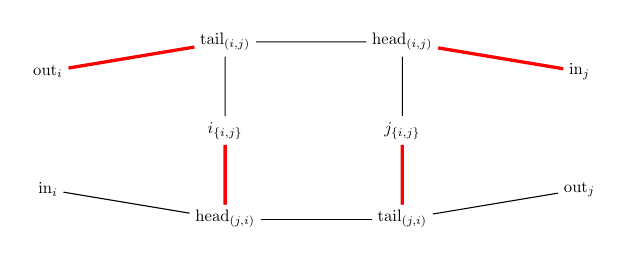
\begin{tikzpicture}[scale=0.75, every node/.style={scale=0.6}]
        \DrawGadget
        \draw[red, very thick] (outi) edge (tailij) (headij) edge (inj) (iij) edge (headji) (jij) edge (tailji);
      \end{tikzpicture}
      \caption{$(i, v_{(i,j)}), (v_{(i,j)}, j) \in \tilde{C}$}
    \end{subfigure}
    \vspace{0.5cm}

    \begin{subfigure}[b]{0.48\textwidth}
      \centering
      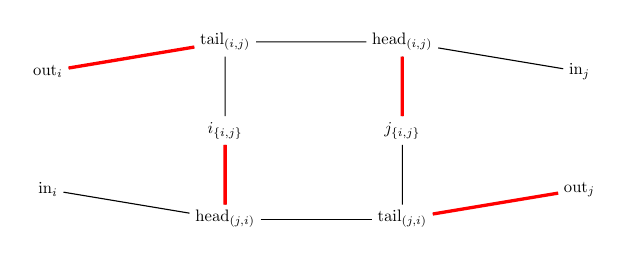
\begin{tikzpicture}[scale=0.75, every node/.style={scale=0.6}]
        \DrawGadget
        \draw[red, very thick] (outi) edge (tailij) (tailji) edge (outj) (iij) edge (headji) (jij) edge (headij);
      \end{tikzpicture}
      \caption{$(i, v_{(i,j)}), (j, v_{(j,i)}) \in \tilde{C}$}
    \end{subfigure}
    \hfill
    \begin{subfigure}[b]{0.48\textwidth}
      \centering
      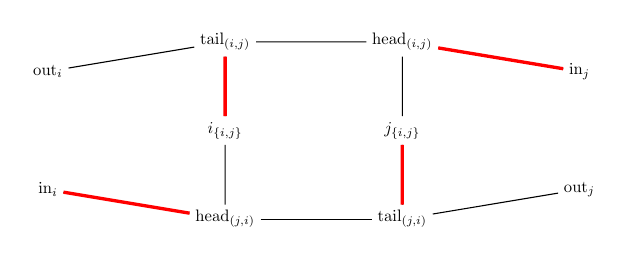
\begin{tikzpicture}[scale=0.75, every node/.style={scale=0.6}]
        \DrawGadget
        \draw[red, very thick] (ini) edge (headji) (headij) edge (inj) (iij) edge (tailij) (jij) edge (tailji);
      \end{tikzpicture}
      \caption{$(v_{(i,j)}, j), (v_{(j,i)}, i) \in \tilde{C}$}
    \end{subfigure}
  \end{figure}
  Łatwo sprawdzić, że skojarzenia doskonałe w grafie $G'$ odpowiadają pokryciom.
\end{proof}

\begin{lemma}
  Niech $\tilde{C}$ będzie pokryciem cyklowym bez 2-cykli, ale z półkrawędziami, dla grafu $G$. W czasie wielomianowym, można skonstruować trzy zbiory rozłącznych wierzchołkowo ścieżek $\mathcal{P}_1$, $\mathcal{P}_2$, $\mathcal{P}_3$, o sumarycznej wadze równej $2w(\tilde{C})$.
\end{lemma}
\begin{proof}
  Niech $F$ będzie zbiorem skierowanych i nieskierowanych krawędzi, powstałym z $\tilde{C}$ w następujący sposób. Dla każdej pary wierzchołków $i, j \in V$, jeśli $(i, v_{(i,j)})$ i $(v_{(i,j)}, j)$ należą do $\tilde{C}$, to do zbioru $F$ dodajemy krawędź skierowaną $(i, j)$. Jeśli natomiast do zbioru $\tilde{C}$ należą $(i, v_{(i,j)})$ i $(j, v_{(j,i)})$, albo $(v_{(i,j)}, j)$ i $(v_{(j,i)}, i)$, to do zbioru $F$ dodajemy krawędź nieskierowaną $\{i,j\}$.

  Skonstruujemy trzy zbiory ścieżek $\mathcal{P}_1$, $\mathcal{P}_2$, $\mathcal{P}_3$, takie że każda krawędź $(i, j) \in F$ występuje w dokładnie dwóch zbiorach, a każda krawędź $\{i,j\} \in F$ występuje raz jako $(i, j)$ w jednym zbiorze oraz raz jako $(j, i)$ w innym zbiorze. Łatwo zauważyć, że sumaryczna waga tych zbiorów to będzie dokładnie $2w(\tilde{C})$.

  Niech $F'$ będzie słabo spójną składową grafu $(V, F)$. Jeśli zignorujemy skierowanie krawędzi, to $F'$ jest cyklem rozmiaru co najmniej $3$. Ponadto, liczba nieskierowanych krawędzi w $F'$ jest parzysta, a skierowane ścieżki (być może puste) po obu stronach każdej nieskierowanej krawędzi mają przeciwną orientację.

  Jeśli $F'$ nie zawiera nieskierowanych krawędzi, to jest skierowanym cyklem. W takim przypadku, niech $e_1, e_2 \in F'$ będą dowolnie wybranymi krawędziami. Do $\mathcal{P}_1$ dodajemy ścieżkę $\{e_1, e_2\}$, do $\mathcal{P}_2$ dodajemy ścieżkę $F' \setminus \{e_1\}$, a do $\mathcal{P}_3$ dodajemy ścieżkę $F' \setminus \{e_2\}$.

  Załóżmy teraz, że $F'$ zawiera jakieś nieskierowane krawędzie. W tej sytuacji, do $\mathcal{P}_1$ dodajemy krawędzie skierowane zgodnie ze wskazówkami zegarami oraz nieskierowane krawędzie, które także kierujemy zgodnie ze wskazówkami zegara.
  Analogicznie, do $\mathcal{P}_2$ dodajemy tak samo powstałe ścieżki, ale dla skierowania przeciwnego do wskazówek zegara.
  Do $\mathcal{P}_3$ dodajemy wszystkie skierowane krawędzie i tylko je.

  Powyższa konstrukcja nie działa jeśli $F'$ jest nieskierowanym cyklem lub skierowane krawędzie tworzą jedną ścieżkę.
  W przypadku gdy $F'$ jest nieskierowanym cyklem, zarówno do $\mathcal{P}_1$ jak i $\mathcal{P}_2$ dodamy cykl.
  W przypadku gdy $F'$ zawiera jeden skierowany segment, to do dokładnie jednego z tych zbiorów dodamy cykl.
  Oryginalny dowód w pracy proponuje coś, co wydaje się bezsensowne: wybieramy dowolną nieskierowaną krawędź i odwracamy jej kierunek w $\mathcal{P}_1$ i $\mathcal{P}_2$. Taki zabieg usuwa cykl skierowany, ale nie zapewnia że są to zbiory rozłącznych wierzchołkowo ścieżek.

  Problem ten jednak łatwo naprawić inaczej. W przypadku, gdy $F'$ zawiera jeden skierowany segment, wybieramy dowolną krawędź nieskierowaną $F'$, i przenosimy ją z odpowiedniego $\mathcal{P}_i$ do $\mathcal{P}_3$. Podobnie, gdy $F'$ jest nieskierowanym cyklem, wybieramy dwie krawędzie nieskierowane, które nie mają wspólnego końca, i przenosimy jedną z nich z $\mathcal{P}_1$ do $\mathcal{P}_3$, a drugą z $\mathcal{P}_2$ do $\mathcal{P}_3$. Zawsze możemy wybrać takie krawędzie, bo jeśli $F'$ jest nieskierowanym cyklem, to ma co najmniej cztery krawędzie.
\end{proof}

\begin{theorem}
  Istnieje algorytm $2/3$-aproksymacyjny dla problemu \textsc{Max-ATSP}. W szczególności, algorytm ten znajduje ścieżkę, której waga to co najmniej $2/3$ optymalnego rozwiązania \textsc{Max-ATSP}.
\end{theorem}

\begin{proof}
  Znajdujemy pokrycie cyklowe bez 2-cykli, ale z półkrawędziami, korzystając z Lematu 1. Następnie budujemy zbiory ścieżek korzystając z Lematu 2. Wybieramy zbiór ścieżek $\mathcal{P}_i$ o największej wadze, i zwracamy dowolną ścieżkę, która zawiera wszystkie krawędzie $\mathcal{P}_i$.
\end{proof}

\section{5/2-aproksymacja dla najkrótszego nadsłowa}

W problemie najkrótszego nadsłowa, mamy dany zbiór słów $S = \{s_1, \ldots, s_n\}$, i chcemy znaleźć najkrótsze słowo $s$, które zawiera wszystkie $s_i$. Zakładamy dla uproszczenia, że zbiór $S$ nie zawiera słowa $s_i$, które jest podsłowem innego słowa $s_j$, dla $i \neq j$.

Dla słów $s$ i $t$, definiujemy nakładkę $\ov(s, t)$ jako najdłuższe słowo $y$ takie że $s = xy$ i $t = yz$, dla pewnych niepustych słów $x$ oraz $z$. Przez $\pref(s, t)$ oznaczamy słowo $x$, tzn. słowo $s$ po usunięciu sufiksu $\ov(s, t)$. Dla ustalonej kolejności słów $s_1, ..., s_n$, najkrótsze nadsłowo to:
\begin{equation*}
	\pref(s_1, s_2)\pref(s_2, s_3)\ldots\pref(s_{n-1}, s_n)\pref(s_n, s_1)\ov(s_n, s_1)
\end{equation*}

Redukcja problemu najkrótszego nadsłowa do problemu \textsc{Max-ATSP-Path} przebiega następująco:
\begin{enumerate}[noitemsep]
	\item Niech $G = (S, E)$ będzie grafem takim że $w(s_i, s_j) = \abs{\pref(s_i, s_j)}$.
	\item Znajdź pokrycie cyklowe $C$ grafu $G$ o najmniejszym koszcie.
	\item Zbuduj zbiór reprezentantów $R$. Dla każdego cyklu tworzymy jednego reprezentata w $R$: jest nim najkrótsze nadsłowo, które zawiera słowa w kolejności występowania na cyklu (wybieramy najlepsze z możliwych rozcięć cyklu).
	\item Niech $G' = (R, E')$ będzie grafem takim że $w(r_i, r_j) = \abs{\ov(r_i, r_j)}$ dla $r_i, r_j \in R$.
	\item Znajdź $\alpha$-aproksymację dla \textsc{Max-ATSP-Path} w grafie $G'$. Niech $P$ będzie kolejnością wierzchołków na znalezionej ścieżce.
	\item Zwróć najkrótsze nadsłowo, które zawiera słowa w kolejności zgodnej z $P$.
\end{enumerate}

Kroki 1-3 mają na celu znalazienie zbioru nadsłów $R$ o tej własności, że słowa mają nieduże nakładki. W krokach 4-6 używamy algorytmu dla \text{Max-ATSP-Path} by znaleźć kolejność słów $R$, dla której słowa najbardziej na siebie nachodzą. Łatwo zauważyć, że gdyby słowa w zbiorze $R$ miały duże nakładki, to aproksymacja w krokach 3-6 nie dawałaby dobrej aproksymacji dla najkrótszego nadsłowa $R$. Okazuje się, że zbiór reprezentantów  wybrany tak jak powyżej daje następującą aproksymację:
\begin{theorem}[\cite{Breslauer1997,Mucha2007}]
  Powyższy algorytm jest $\left(\frac{7}{2}-\frac{3}{2}\alpha\right)$-aproksymacyjny dla problemu najkrótszego nadsłowa.
\end{theorem}

Przystępne opracowanie tej redukcji wraz z dowodami można znaleźć w \cite{Mucha2007}. Podstawiając $\alpha = 2/3$ dostajemy ostateczny wynik:

\begin{theorem}
  Istnieje algorytm $5/2$-aproksymacyjny dla problemu najkrótszego nadsłowa.
\end{theorem}

\begin{thebibliography}{}
  \bibitem{Paluch2012}{Paluch, Katarzyna, Khaled Elbassioni, and Anke Van Zuylen. "Simpler approximation of the maximum asymmetric traveling salesman problem." STACS'12 (29th Symposium on Theoretical Aspects of Computer Science). Vol. 14. LIPIcs, 2012.}
  \bibitem{Breslauer1997}{Breslauer, Dany, Tao Jiang, and Zhigen Jiang. "Rotations of periodic strings and short superstrings." Journal of Algorithms 24.2 (1997): 340-353.}
  \bibitem{Blaser2002}{Bläser, Markus, and Bodo Manthey. "Two approximation algorithms for 3-cycle covers." International Workshop on Approximation Algorithms for Combinatorial Optimization. Springer, Berlin, Heidelberg, 2002.}
  \bibitem{Mucha2007}{Mucha, Marcin. "A tutorial on shortest superstring approximation." (2007).}
\end{thebibliography}

\end{document}
